\documentclass[11pt]{article}
\usepackage{bm}
\usepackage{ctex}
\usepackage{array}
\usepackage{color}
\usepackage{float}
\usepackage{xcolor}
\usepackage{amssymb}
\usepackage{amsmath}
\usepackage{graphicx}
\usepackage{listings}
\usepackage{tabularx}
\usepackage{hyperref}
\usepackage{fancyhdr}
\usepackage{enumitem}
\usepackage{enumerate}
\definecolor{keywordcolor}{rgb}{0.8,0.1,0.5}

\pagestyle{fancy}
\hypersetup{hypertex = true,
			colorlinks = false,
			linkcolor = blue ,
			anchorcolor = blue,
			citecolor = blue}
\fancyhf{}


\definecolor{mygreen}{rgb}{0,0.6,0}  
\definecolor{mygray}{rgb}{0.5,0.5,0.5}  
\definecolor{mymauve}{rgb}{0.58,0,0.82}  

\lstset{ %  
	backgroundcolor=\color{white},   % choose the background color; you must add \usepackage{color} or \usepackage{xcolor}  
	basicstyle=\footnotesize,        % the size of the fonts that are used for the code  
	breakatwhitespace=false,         % sets if automatic breaks should only happen at whitespace  
	breaklines=true,                 % sets automatic line breaking  
	captionpos=bl,                    % sets the caption-position to bottom  
	commentstyle=\color{mygreen},    % comment style  
	deletekeywords={...},            % if you want to delete keywords from the given language  
	escapeinside={\%*}{*)},          % if you want to add LaTeX within your code  
	extendedchars=true,              % lets you use non-ASCII characters; for 8-bits encodings only, does not work with UTF-8  
	frame=single,                    % adds a frame around the code  
	keepspaces=true,                 % keeps spaces in text, useful for keeping indentation of code (possibly needs columns=flexible)  
	keywordstyle=\color{blue},       % keyword style  
	%language=Python,                 % the language of the code  
	morekeywords={*,...},            % if you want to add more keywords to the set  
	numbers=none,                    % where to put the line-numbers; possible values are (none, left, right)  
	numbersep=5pt,                   % how far the line-numbers are from the code  
	numberstyle=\tiny\color{mygray}, % the style that is used for the line-numbers  
	rulecolor=\color{black},         % if not set, the frame-color may be changed on line-breaks within not-black text (e.g. comments (green here))  
	showspaces=false,                % show spaces everywhere adding particular underscores; it overrides 'showstringspaces'  
	showstringspaces=false,          % underline spaces within strings only  
	showtabs=false,                  % show tabs within strings adding particular underscores  
	stepnumber=1,                    % the step between two line-numbers. If it's 1, each line will be numbered  
	stringstyle=\color{orange},     % string literal style  
	tabsize=3,                       % sets default tabsize to 2 spaces  
	%title=myPython.py                   % show the filename of files included with \lstinputlisting; also try caption instead of title  
}

\chead{Compiler}
\fancyhead[r]{\bfseries\thepage}
\fancyhead[l]{\bfseries\rightmark}
\setlength{\listparindent}{0em} %段落缩进量
\begin{titlepage}
	\title{05-12编译原理作业11}
	\author{
			\textbf{作者:} {吴润泽}
			\and {\textbf{学号:} 181860109}
		}
\end{titlepage}
\begin{document}
\maketitle
\section*{7.5.2}

\begin{table}[H]
	\centering
	\label{tab:752}
	\resizebox{\textwidth}{!}{%
		\begin{tabular}{|c|c|c|c|c|c|c|c|c|c|}
			\hline
			\textbf{对象} & \textbf{A} & \textbf{B} & \textbf{C} & \textbf{D} & \textbf{E} & \textbf{F} & \textbf{G} & \textbf{H} & \textbf{I} \\ \hline
			删除前引用计数     & 1          & 1          & 1          & 1          & 3          & 1          & 1          & 3          & 3          \\ \hline
			删除后引用计数     & 1          & 1          & 1          & 0          & 3          & 0          & 0          & 1          & 2          \\ \hline
		\end{tabular}%
	}
\end{table}

\noindent$D,F,G,I$引用计数减1,$H$引用计数减2。其中$D,F,G$计数变为0,故将其删去,删除后的结果如下图所示。
\begin{figure}[H]
	\centering
	\label{fig:7.5.1}
	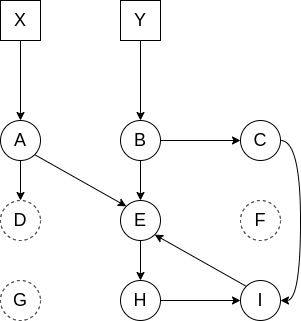
\includegraphics[scale=0.55]{7.6.1.png}
	\caption{删除后的引用情况}
\end{figure}
\section*{7.6.1}
\subsection*{3)删除A$\rightarrow$D}
\begin{lstlisting}
	a. 初始化:	A.reached=...=I.reached=0
	b. 标记阶段:
		line1:	A,B作为根集
					Unscanned=[A,B] A.reached=B.reached=1
		line2-7:		BFS遍历标记
			loop1:	Unscanned=[B,E] E.reached=1
			loop2:	Unscanned=[E,C] C.reached=1
			loop3:	Unscanned=[C,H] H.reached=1
			loop4:	Unscanned=[H,I] I.reached=1
			loop5:	Unscanned=[I]
			loop6:	Unscanned=[]
	c. 清扫阶段:
		line8:		Free=[]
		line9-11:	Free=[D,F,G] A.reached=...=I.reached=0
\end{lstlisting}
删除后的结果与\hyperref[fig:7.5.1]{图1}相同。
\end{document}